\chapter{AsthmaBuddy Manual}
\label{app:asthmabuddy_manual}

The following Appendix works as a user manual for AsthmaBuddy.

\section{Introduction}
The source code is specifically written to be run on a \rpi{}. As such, the program WILL NOT work on other computers.

\subsection{Dependencies}
\label{sec:dependencies} 
We have used a couple of frameworks in order to make the development process easier. Downloading and placing them in the correct folder is important in order to compile and run the application. 

\paragraph{Java}
As of September 2013, all \rpi{}s are shipped with Java by default. If your version of \rpi{} was bought before this, Java can be downloaded and installed through this command: 

\code{sudo apt-get update \&\& sudo apt-get install oracle-java7-jdk}

\paragraph{Pi4J}
Pi4J can be downloaded from the following URL: \url{http://pi4j.com}. To install it, simply follow the installation guide at the same page\fnurl{Pi4J Installation guide}{http://pi4j.com/install.html}. 

\paragraph{Google Gson}
Google's Gson can be downloaded from the following URL: \url{https://code.google.com/p/google-gson/downloads/list}. Put it in the folder \code{/home/pi/Downloads/}. 
The path to gson-2.2.4.jar should be \code{/home/pi/Downloads/google-gson-2.2.4/gson-2.2.4.jar}.

\paragraph{JLayer}
JLayer can be downloaded the following URL: \url{http://www.javazoom.net/javalayer/javalayer.html}. Put the file \code{jl1.0.1.jar} in the folder \code{/home/pi/jlayer/JLayer1.0.1/}, which should make the path to the file \code{/home/pi/jlayer/JLayer1.0.1/jl1.0.1.jar}.  

\paragraph{Joda Time}
Joda Time can be downloaded from the following URL: \url{http://www.joda.org/joda-time/}. Put the file \code{joda-time-2.3.jar} in the folder \code{/home/pi/Downloads/joda-time-2.3}, which should make the path to the file \code{/home/pi/Downloads/joda-time-2.3/joda-time-2.3.jar}. 

\paragraph{Node.js}
Node.js can be downloaded from the following URL: \url{http://nodejs.org/}. Finding the source code for our Node.js server is found in Section \ref{sec:sourcecode}

\section{GPIO setup}
In order for \ab{} to work properly, you need to use an RGB LED diode, which is connected to the \rpi{} through the GPIO pins. This section will elaborate on the details of this process. 

Figure \ref{fig:rgb-led} shows the RGB LED-diode we used to emit light signals. As you can see, there are four pins: Blue (1), Ground(2), Green(3) and Red(4). Pins 1,3 and 4 are connected to a 220 Ohm Resistor. Figure \ref{fig:rpigpio} shows an overview of the available Gpio ports.  Table \ref{tab:wiringgpio} shows how the pins are then wired to the \rpi{}. 

\begin{figure}
	\begin{minipage}[t]{0.4\linewidth}
		\centering
			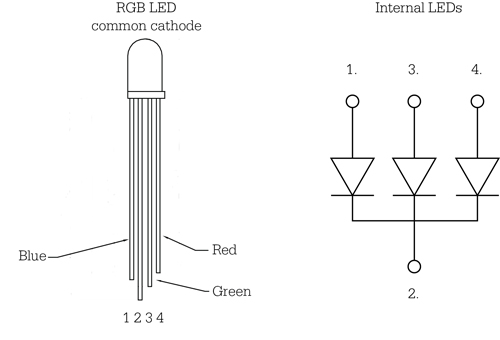
\includegraphics[width=0.30\paperwidth]{Pictures/rgb_led_diagram.jpg}
		\caption{RGB LED diagram. [INSERT IMAGE SOURCE]}
		\label{fig:rgb-led}
	\end{minipage}
	\hspace{1cm}
	\begin{minipage}[t]{0.4\linewidth}
		\centering
			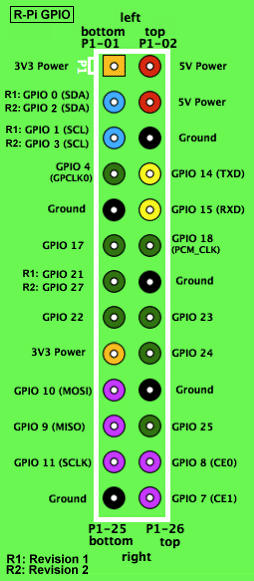
\includegraphics[width=0.20\paperwidth]{Pictures/GPIOs.png}
		\caption{\rpi{} GPIO. [INSERT IMAGE SOURCE]}
		\label{fig:rpigpio}
	\end{minipage}
\end{figure}

\begin{table}[H]
\centering
\begin{tabular}{|p{3.0cm}| p{3.0cm}|}
	\hline
	\textbf{LED Pin} & \textbf{Wired to GPIO port}\\
	\hline
	Blue (1) & GPIO 17\\
	\hline
	Ground (2) & Ground\\
	\hline
	Green (3) & GPIO 18\\
	\hline
	Red (4) & GPIO 21/27 (Revision 1/Revision 2)\\
	\hline
\end{tabular}
\caption{Wiring LED pins to GPIO}
\label{tab:wiringgpio}
\end{table}

\section{RFID reader}
We used the Sparkfun ID-12LA RFID-reader. This was connected through the bottom USB port on the \rpi{}. 
The application needs the port name of the USB reader. This can be found by the following command: 

\code{ls /dev | grep USB}

If the output is not equal to \code{/dev/ttyUSB0}, you can insert your name in the variable \code{comPort} in the file \code{src/com/blopp/pi/readers/RFIDReader.java}. 
 
\section{Source code}
\label{sec:sourcecode}
[TODO: Wait for clarification from Pieter, Ole and Elin]
[TODO: Remember the node server]


\section{Running AsthmaBuddy}

\subsection{Compiling}
If the guide in \ref{sec:dependencies} was followed carefully enough, the program can be compiled by running:

\code{./src/compile.sh}

Alternatively, you may extract the exact command from \code{compile.sh}, and run it directly from the terminal window. 

\subsection{Running}
The program can run by using the following script:

\code{./src/v2.sh}

Alternatively, you may extract the exact command from \code{v2.sh}, and run it directly from the terminal window. 

\paragraph{Parameters}

Once the program is running, it checks for alarms stored for the user. 

Once the message \emph{``Did not find any alarms''} appears, you can type in parameters on this format: \emph{CN}. 

C is the color of the medicine that is to be taken. C $\in \{ b = Blue, o = Orange, p = Purple \}$.

N is the interaction method you want to use. N $\in \{ 0, 1, 3, 4, 6, 9\}$. The interaction methods provided are summarized in Table \ref{tab:interactionmethodsguide}.

An example on a valid input is:

\code{b1}

\begin{table}[H]
\begin{tabular}{|p{3.0cm} | p{7.0cm}|}
\hline
\textbf{N} & \textbf{Interaction method} \\
\hline
0 & \emph{Clap your hands} \\
\hline
1 & \emph{Variation of those provided in this table} \\
\hline
3 & \emph{Hold \ab{}'s hand to proceed} \\
\hline
4 & \emph{Hold your card against \ab{}'s stomach}\\
\hline
6 & \emph{Give an high five} \\
\hline
9 & \emph{Press \ab{}'s stomach} \\
\hline
\end{tabular}
\caption{Guide for interactions in \ab{}.}
\label{tab:interactionmethodsguide}
\end{table}

After this, you can press \emph{Enter} every time the user has interacted with \ab{}, and the windows says \emph{Ready for User Input}. 